\documentclass{article}[18pt]
\ProvidesPackage{format}
%Page setup
\usepackage[utf8]{inputenc}
\usepackage[margin=0.7in]{geometry}
\usepackage{parselines} 
\usepackage[english]{babel}
\usepackage{fancyhdr}
\usepackage{titlesec}
\hyphenpenalty=10000

\pagestyle{fancy}
\fancyhf{}
\rhead{Sam Robbins}
\rfoot{Page \thepage}

%Characters
\usepackage{amsmath}
\usepackage{amssymb}
\usepackage{gensymb}
\newcommand{\R}{\mathbb{R}}

%Diagrams
\usepackage{pgfplots}
\usepackage{graphicx}
\usepackage{tabularx}
\usepackage{relsize}
\pgfplotsset{width=10cm,compat=1.9}
\usepackage{float}

%Length Setting
\titlespacing\section{0pt}{14pt plus 4pt minus 2pt}{0pt plus 2pt minus 2pt}
\newlength\tindent
\setlength{\tindent}{\parindent}
\setlength{\parindent}{0pt}
\renewcommand{\indent}{\hspace*{\tindent}}

%Programming Font
\usepackage{courier}
\usepackage{listings}
\usepackage{pxfonts}

%Lists
\usepackage{enumerate}
\usepackage{enumitem}

% Networks Macro
\usepackage{tikz}


% Commands for files converted using pandoc
\providecommand{\tightlist}{%
	\setlength{\itemsep}{0pt}\setlength{\parskip}{0pt}}
\usepackage{hyperref}

% Get nice commands for floor and ceil
\usepackage{mathtools}
\DeclarePairedDelimiter{\ceil}{\lceil}{\rceil}
\DeclarePairedDelimiter{\floor}{\lfloor}{\rfloor}

% Allow itemize to go up to 20 levels deep (just change the number if you need more you madman)
\usepackage{enumitem}
\setlistdepth{20}
\renewlist{itemize}{itemize}{20}

% initially, use dots for all levels
\setlist[itemize]{label=$\cdot$}

% customize the first 3 levels
\setlist[itemize,1]{label=\textbullet}
\setlist[itemize,2]{label=--}
\setlist[itemize,3]{label=*}

% Definition and Important Stuff
% Important stuff
\usepackage[framemethod=TikZ]{mdframed}

\newcounter{theo}[section]\setcounter{theo}{0}
\renewcommand{\thetheo}{\arabic{section}.\arabic{theo}}
\newenvironment{important}[1][]{%
	\refstepcounter{theo}%
	\ifstrempty{#1}%
	{\mdfsetup{%
			frametitle={%
				\tikz[baseline=(current bounding box.east),outer sep=0pt]
				\node[anchor=east,rectangle,fill=red!50]
				{\strut Important};}}
	}%
	{\mdfsetup{%
			frametitle={%
				\tikz[baseline=(current bounding box.east),outer sep=0pt]
				\node[anchor=east,rectangle,fill=red!50]
				{\strut Important:~#1};}}%
	}%
	\mdfsetup{innertopmargin=10pt,linecolor=red!50,%
		linewidth=2pt,topline=true,%
		frametitleaboveskip=\dimexpr-\ht\strutbox\relax
	}
	\begin{mdframed}[]\relax%
		\centering
		}{\end{mdframed}}



\newcounter{lem}[section]\setcounter{lem}{0}
\renewcommand{\thelem}{\arabic{section}.\arabic{lem}}
\newenvironment{defin}[1][]{%
	\refstepcounter{lem}%
	\ifstrempty{#1}%
	{\mdfsetup{%
			frametitle={%
				\tikz[baseline=(current bounding box.east),outer sep=0pt]
				\node[anchor=east,rectangle,fill=blue!20]
				{\strut Definition};}}
	}%
	{\mdfsetup{%
			frametitle={%
				\tikz[baseline=(current bounding box.east),outer sep=0pt]
				\node[anchor=east,rectangle,fill=blue!20]
				{\strut Definition:~#1};}}%
	}%
	\mdfsetup{innertopmargin=10pt,linecolor=blue!20,%
		linewidth=2pt,topline=true,%
		frametitleaboveskip=\dimexpr-\ht\strutbox\relax
	}
	\begin{mdframed}[]\relax%
		\centering
		}{\end{mdframed}}
\lhead{ADS - Part 4}


\begin{document}
\begin{center}
\underline{\huge Minimum Spanning Trees}
\end{center}
\section{Connecting the vertices}
Input: a graph G=(V,E) with a weight (or a cost) w(u,v) for each edge (u,v)
\begin{center}
	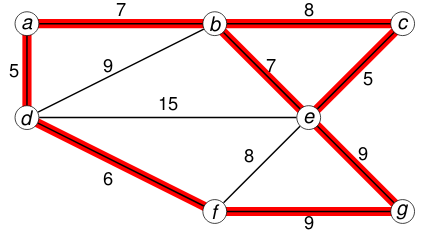
\includegraphics[scale=0.7]{graph1}
\end{center}
Objective: Choose a subset of the edges that connects the vertices. Find the solution that costs the least
\subsection{Minimum spanning tree problem}
\begin{center}
	\textit{Find a tree that spans the vertices and has minimum cost}
\end{center}
Basic properties of MSTs:
\begin{itemize}
	\item have $|V|-1$ edges
	\item Have no cycles
	\item might not be unique
\end{itemize}
\section{Representations of weighted graphs}
$$\left( \begin{array} { c c c c c c c c c } { 0 } & { 5 } & { 0 } & { 4 } & { 0 } & { 0 } & { 0 } & { 0 } & { 0 } \\ { 5 } & { 0 } & { 10 } & { 3 } & { 9 } & { 0 } & { 0 } & { 0 } & { 0 } \\ { 0 } & { 10 } & { 0 } & { 0 } & { 5 } & { 7 } & { 0 } & { 0 } & { 0 } \\ { 4 } & { 3 } & { 0 } & { 0 } & { 8 } & { 0 } & { 7 } & { 0 } & { 0 } \\ { 0 } & { 9 } & { 5 } & { 8 } & { 0 } & { 7 } & { 6 } & { 7 } & { 0 } \\ { 0 } & { 0 } & { 7 } & { 0 } & { 7 } & { 0 } & { 0 } & { 2 } & { 4 } \\ { 0 } & { 0 } & { 0 } & { 7 } & { 6 } & { 0 } & { 0 } & { 5 } & { 0 } \\ { 0 } & { 0 } & { 0 } & { 0 } & { 7 } & { 2 } & { 5 } & { 0 } & { 3 } \\ { 0 } & { 0 } & { 0 } & { 0 } & { 0 } & { 4 } & { 0 } & { 3 } & { 0 } \end{array} \right)$$
Note that the zeros represent the fact there is no edge between the two nodes, it could equally be $\infty$
\begin{center}
	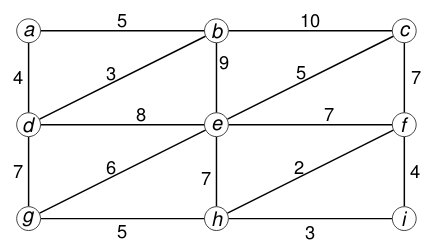
\includegraphics[scale=0.7]{graph2}
\end{center}
\section{Kruskal's Algorithm}
\begin{enumerate}
	\item Sort the edges by weight
	\item Let A=$\varnothing$
	\item Consider edges in increasing order of weight. For each edge e, add e to A unless this would create a cycle (cycles are detected by running BFS between the two vertices before joining them, however this is a naive method)
\end{enumerate}
Running time is $\mathcal{O}(E\log V)$
\begin{center}
	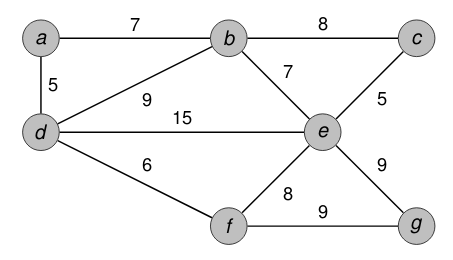
\includegraphics[scale=0.7]{graph3}
\end{center}
\subsection{Correctness}
\textbf{Claim} - The set A is always a subtree of an MST\\
The claim implies the algorithm is correct since when it terminates, A is a spanning tree.\\
\\
\textbf{Proof of the claim} - By induction\\
\textbf{Base case}
\begin{itemize}
	\item $A=\varnothing$ so the claim is true in this case
\end{itemize}
\textbf{Inductive step}:
\begin{itemize}
	\item Assume A is a subtree of a MST
	\item Must show that $A+e$ us a subtree of a MST when e is added to A.
	\item Let T be the MST that contains A
	\item If T contains $e$, we are done
	\item Suppose $e$ is not in T. So $T+e$ contains a cycle
	\item Some of the edges in the cycle are not in $A+e$
	\item Let f be an edge in the cycle not in $A+e$
	\item Consider $T+e-f$. A tree that contains $A+e$
	\item $w(T+e-f)> w(T)$ since T is an MST
	\item $w(T)+w(e)-w(F)> w(T)$
	\item $w(e)>w(F)$
	\item This is a contradiction. The algorithm should pick $F$ before $e$
\end{itemize}


\section{Prim's Algorithm}
\begin{enumerate}
	\item Let $U=\{u\}$ where u is some vertex chosen arbitrarily
	\item Let $A=\varnothing$
	\item Until U contains all vertices: find the least weight edge e that joins a vertex v in U to a vertex w not in U and add e to A and w to U
\end{enumerate}
Running time is $\mathcal{O}(V\log V+E)$
\subsection{Correctness}
\begin{itemize}
	\item Let T be the output
	\item Suppose that T is not a MST
	\item Let $T^*$ be a MST with most edges in common with T
	\item Let e be the first edge that belongs to T but not $T^*$
	\item Consider the moment that $e$ is chosen
	\begin{itemize}
		\item U is the vertices chosen so far
		\item W is the remaining vertices
		\item Let e connect U to W
		\item $T^*$ must contain some other edge f from U to W
		\item And $w(f)\geqslant w(e)$
	\end{itemize}
	\item Notice that $T^*+e-f$ is a tree
	\item $w(T^*+e-f)\leqslant w(T^*)$
	\item So $w(T^*+e-f)=w(T^*)$ as no spanning trees can weigh less than $T^*$ as it is an MST
	\item So $T^*+e-f$ is a MST with more edges in common with T than $T^*$
	\item A contradiction. BAM.
\end{itemize}
\end{document}